%!TEX program = xelatex

\documentclass[12pt]{report}

\usepackage[utf8]{inputenc}
\usepackage{lipsum}
\usepackage{amsmath}
\usepackage{amssymb}
\usepackage{amsthm}
\usepackage{graphicx}
\usepackage{setspace}
\usepackage{caption}
\usepackage{subcaption}
\usepackage{float}
\usepackage[top=38mm,left=38mm,bottom=25mm,right=25mm]{geometry}
\usepackage{listings}
\usepackage{textcomp}
\usepackage{multicol}
\usepackage[toc,page]{appendix}
\usepackage{listings}
\usepackage{fancyvrb}
\usepackage{hyperref}
\usepackage{etoolbox}

\usepackage[displaymath, mathlines, pagewise]{lineno}
\renewcommand\linenumberfont{\normalfont\scriptsize\rmfamily}

\usepackage{lstbayes}
\usepackage{subfiles}
\usepackage{fancyhdr}
\usepackage{booktabs}
\usepackage[section]{placeins}

\pagestyle{fancy}
\fancyhead{}
\fancyhead[LE,RO]{McMaster University - Mathematics}
\fancyhead[LO,RE]{M.Sc. Thesis - Dexter Barrows}
\fancyfoot{}
\fancyfoot[C]{\thepage}
%\renewcommand{\footrulewidth}{0.4pt}% default is 0pt

%\setlength{\belowcaptionskip}{-10pt}

\usepackage[backend=biber]{biblatex}
\addbibresource{thesis-refs.bib}

\usepackage[dvipsnames]{xcolor}
\definecolor{DGrey}{gray}{0.25}
\definecolor{MGrey}{gray}{0.50}
\definecolor{LGrey}{gray}{0.75}

\hypersetup{%
  colorlinks=false,
  linkbordercolor=red
}

\usepackage[ruled,vlined,linesnumbered]{algorithm2e}
\newcommand\mycommfont[1]{\footnotesize\ttfamily\textcolor{gray}{#1}}
\SetCommentSty{mycommfont}

\usepackage{inconsolata}

\usepackage[parfill]{parskip}
\setlength{\parindent}{0pt}
%\setlength{\parskip}{\baselineskip}

\newcommand{\et}{e^{i\theta}}
\newcommand{\oo}{\mathcal{O}}
\newcommand{\skipline}{\bigskip\bigskip\bigskip}

\lstdefinestyle{Rsty} { 
    language=R,                         % the language of the code
    basicstyle=\footnotesize\ttfamily,  % the size of the fonts that are used for the code
    numbers=left,                       % where to put the line-numbers
    numberstyle=\footnotesize\color{LGrey},      % the style that is used for the line-numbers
    stepnumber=1,                       % the step between two line-numbers. If it is 1, each line
                                        % will be numbered
    numbersep=5pt,                      % how far the line-numbers are from the code
    backgroundcolor=\color{white},      % choose the background color. You must add \usepackage{color}
    showspaces=false,                   % show spaces adding particular underscores
    showstringspaces=false,             % underline spaces within strings
    showtabs=false,                     % show tabs within strings adding particular underscores
    frame=single,                       % adds a frame around the code
    rulecolor=\color{black},            % if not set, the frame-color may be changed on line-breaks within not-black text (e.g. commens (green here))
    tabsize=2,                          % sets default tabsize to 2 spaces
    captionpos=b,                       % sets the caption-position to bottom
    breaklines=true,                    % sets automatic line breaking
    breakatwhitespace=false,            % sets if automatic breaks should only happen at whitespace
    keywordstyle=\color{DGrey},     % keyword style
    commentstyle=\color{LGrey},   % comment style
    stringstyle=\color{MGrey},    % string literal style
    literate={<-}{{$\gets$}}1,           % prettier assignment arrows
    xleftmargin=4.0ex,
    deletekeywords={I,density,rect,_,palette,data,scale,panel,R,frame,labels,options}
}

\lstnewenvironment{R}
{\lstset{style=Rsty}}
{}

\lstdefinestyle{Stansty} { 
    language=Stan,                         % the language of the code
    basicstyle=\footnotesize\ttfamily,  % the size of the fonts that are used for the code
    numbers=left,                       % where to put the line-numbers
    numberstyle=\footnotesize\color{LGrey},      % the style that is used for the line-numbers
    stepnumber=1,                       % the step between two line-numbers. If it is 1, each line
                                        % will be numbered
    numbersep=5pt,                      % how far the line-numbers are from the code
    backgroundcolor=\color{white},      % choose the background color. You must add \usepackage{color}
    showspaces=false,                   % show spaces adding particular underscores
    showstringspaces=false,             % underline spaces within strings
    showtabs=false,                     % show tabs within strings adding particular underscores
    frame=single,                       % adds a frame around the code
    rulecolor=\color{black},            % if not set, the frame-color may be changed on line-breaks within not-black text (e.g. commens (green here))
    tabsize=2,                          % sets default tabsize to 2 spaces
    captionpos=b,                       % sets the caption-position to bottom
    breaklines=true,                    % sets automatic line breaking
    breakatwhitespace=false,            % sets if automatic breaks should only happen at whitespace
    keywordstyle=\color{DGrey},     % keyword style
    commentstyle=\color{LGrey},   % comment style
    stringstyle=\color{MGrey},    % string literal style
    %literate={<-}{{$\gets$}}1,           % prettier assignment arrows
    xleftmargin=4.0ex,
    deletekeywords={T}
}

\lstnewenvironment{Stan}
{\lstset{style=Stansty}}
{}

\lstdefinestyle{Cppsty} { 
    language=C++,                         % the language of the code
    basicstyle=\footnotesize\ttfamily,  % the size of the fonts that are used for the code
    numbers=left,                       % where to put the line-numbers
    numberstyle=\footnotesize\color{LGrey},      % the style that is used for the line-numbers
    stepnumber=1,                       % the step between two line-numbers. If it is 1, each line
                                        % will be numbered
    numbersep=5pt,                      % how far the line-numbers are from the code
    backgroundcolor=\color{white},      % choose the background color. You must add \usepackage{color}
    showspaces=false,                   % show spaces adding particular underscores
    showstringspaces=false,             % underline spaces within strings
    showtabs=false,                     % show tabs within strings adding particular underscores
    frame=single,                       % adds a frame around the code
    rulecolor=\color{black},            % if not set, the frame-color may be changed on line-breaks within not-black text (e.g. commens (green here))
    tabsize=4,                          % sets default tabsize to 2 spaces
    captionpos=b,                       % sets the caption-position to bottom
    breaklines=true,                    % sets automatic line breaking
    breakatwhitespace=false,            % sets if automatic breaks should only happen at whitespace
    keywordstyle=\color{DGrey},     % keyword style
    commentstyle=\color{LGrey},   % comment style
    stringstyle=\color{MGrey},    % string literal style
    %literate={<-}{{$\gets$}}1,           % prettier assignment arrows
    xleftmargin=4.0ex,
    deletekeywords={T}
}

\lstnewenvironment{CPP}
{\lstset{style=Cppsty}}
{}

\makeatletter
\let\org@subfile\subfile
\renewcommand*{\subfile}[1]{%
  \filename@parse{#1}% LaTeX's file name parser
  \expandafter
  \graphicspath\expandafter{\expandafter{\filename@area}}%
  \org@subfile{#1}%
}
\makeatother

\renewcommand{\arraystretch}{2}

\begin{document}

	\subfile{halftitle}

	%% --------------------------------------------------------------------

	\subfile{titlepage}

	\setcounter{page}{1}
	\pagenumbering{roman}

	%% --------------------------------------------------------------------

	\subfile{infopage}

	%% --------------------------------------------------------------------

	\chapter*{Abstract}

		Forecasting tools play an important role in public response to epidemics. Despite this, limited work has been done in comparing best-in-class techniques across the broad spectrum of time series forecasting methodologies. Forecasting frameworks were developed that utilised three methods designed to work with nonlinear dynamics: IF2, Hamiltonian MCMC, and S-mapping. These were compared in several forecasting scenarios including a seasonal epidemic and a spatiotemporal epidemic. IF2 combined with parametric bootstrapping produced superior predictions in all scenarios. S-mapping combined with Dewdrop Regression produced forecasts slightly less-accurate than IF2 and HMCMC, but demonstrated vastly reduced running times. Hence, S-mapping with or without Dewdrop Regression should be used to glean initial insight into future epidemic behaviour, while IF2 and parametric bootstrapping should be used to refine forecast estimates in time.


	\chapter*{Acknowledgements}

		There are many people I have to thank for their support over the last two years:

		My supervisor Dr. Ben Bolker for his mentorship, advice, direction, and especially patience.

		My defence committee members Dr. Jonathan Dushoff and Dr. David Earn who have taken the time to read my work and provide valuable input.

		The Theobio lab for including me in stimulating discussions, even when they were over my head.

		My Mom, Dad, Joel, and Sof\'{i}a for being there for me through good times and trying ones.



	\tableofcontents

	\listoffigures

	%% --------------------------------------------------------------------
	%% --------------------------------------------------------------------

	\newpage
	
	\begin{linenumbers}

	\setcounter{page}{1}
	\pagenumbering{arabic}

	\chapter{Introduction}

		\subfile{../introduction/introduction}

	\chapter{Hamiltonian MCMC}

		\subfile{../MCMC-HMCMC/mcmc-text}

	\chapter{Iterated Filtering}

		\graphicspath{{../PF-IF2/}}
		%% Dexter Barrows, 2016
%% dbarrows.github.io

\section{Intro}

	Particle filters are similar to MCMC-based methods in that they attempt to draw samples from an approximation of the posterior distribution of model parameters $\theta$ given observed data $D$. Instead of constructing a Markov chain and approximating its stationary distribution, a cohort of ``particles'' are used to move through the data in an on-line (sequential) fashion with the cohort being culled of poorly-performing particles at each iteration via importance sampling. If the culled particles are not replenished, this will be a Sequential Importance Sampling (SIS) particle filter. If the culled particles are replenished from surviving particles, in a sense setting up a process not dissimilar from Darwinian selection, then this will be a Sequential Importance Resampling (SIR) particle filter.


\section{Formulation}

	Particle filters, also called Sequential Monte-Carlo (SMC) or bootstrap filters, feature similar core functionality as the venerable Kalman Filter. As the algorithm moves through the data (sequence of observations), a prediction-update cycle is used to simulate the evolution of the model $M$ with different particular parameter selections, track how closely these predictions approximate the new observed value, and update the current cohort appropriately.

	Two separate functions are used to simulate the evolution and observation processes. The ``true'' state evolution is specified by

	\begin{equation}
		X_{t+1} \sim f_1 (X_t, \theta),
	\end{equation}

	And the observation process by

	\begin{equation}
		Y_t \sim f_2 (X_t, \theta).
	\end{equation}

	Note that components of $\theta$ can contribute to both functions, but a typical formulation is to have some components contribute to $f_1 (\cdot, \theta)$ and others to $f_2 (\cdot,\theta)$.

	The prediction part of the cycle utilises $f_1 (\cdot, \theta)$ to update each particle's current state estimate to the next time step, while $f_2 (\cdot, \theta)$ is used to evaluate a weighting $w$ for each particle which will be used to determine how closely that particle is estimating the true underlying state of the system. Note that $f_2 (\cdot, \theta)$ could be thought of as a probability of observing a piece of data $y_t$ given the particle's current state estimate and parameter set, $P(y_t | X_t, \theta)$. Then, the new cohort of particles is drawn from the old cohort proportional to the weights. This process is repeated until the set of observations $D$ is exhausted.


\section{Algorithm}

    Now we will formalize the particle filter.

    We will denote each particle $p^{(j)}$ as the $j^{th}$ particle consisting of a state estimate at time $t$, $X_t^{(j)}$, a parameter set $\theta^{(j)}$, and a weight $w^{(j)}$. Note that the state estimates will evolve with the system as the cohort traverses the data.

    The algorithm for a Sequential Importance Resampling particle is shown in Algorithm \ref{pfsir}.\\
    
    \begin{algorithm}[H]

        \BlankLine

        \SetKwInOut{Input}{Input}
        \SetKwInOut{Output}{Output}
        \DontPrintSemicolon

        \tcc{Select a starting point}
        \Input{Observations $D = y_1, y_2, ..., y_T$, initial particle distribution $P_0$ of size $J$}

        \BlankLine

        \tcc{Setup}
        Initialize particle cohort by sampling $(p^{(1)}, p^{(2)}, ..., p^{(J)})$ from $P_0$

        \BlankLine

        \For{$t = 1:T$}{

            \BlankLine

            \tcc{Evolve}
            \For{j = 1:J}{
            	$X_t^{(j)} \gets f_1 (X_{t-1}^{(j)}, \theta^{(j)})$
            }

            \BlankLine

            \tcc{Weight}
            \For{j = 1:J}{
            	$w^{(j)} \gets P(y_t | X_t^{(j)}, \theta^{(j)}) = f_2 (X_t^{(j)}, \theta^{(j)})$
            }

            \BlankLine

            \tcc{Normalize}
            \For{j = 1:J}{
            	$w^{(j)} \gets w^{(j)} / \sum_{1}^{J} w^{(j)}$
            }

            \BlankLine

            \tcc{Resample}
            $p^{(1:J)} \gets \text{sample}(p^{(1:J)}, \text{prob} = w, \text{replace} = true)$
        }

        \BlankLine

        \tcc{Samples from approximated posterior distribution}
        \Output{Cohort of posterior samples $(\theta^{(1)},\theta^{(2)},...,\theta^{(J)})$}

        \BlankLine

        \caption{SIR particle filter}\label{pfsir}

    \end{algorithm}

\section{Particle Collapse}

	Not uncommonly, a situation may arise in which a single particle is assigned a normalized weight very close to 1 and all the other particles are assigned weights very close to 0. When this occurs, the next generation of the cohort will overwhelmingly consist of descendants of the heavily-weighted particle, termed particle collapse or degeneracy.

	Since the basic SIR particle filter does not perturb either the particle system states or system parameter values, the cohort will quickly consist solely of identical particles, effectively halting further exploration of the parameter space as new data is introduced.

	A similar situation occurs when a small number of particles (but not necessarily a single particle) split almost all of the normalized weight between them, then jointly dominate the resampling process for the remainder of the iterations. This again halts the exploration of the parameter space with new data.

	In either case, the hallmark feature used to detect collapse is the same -- at some point the cohort will consist of particles with very similar or identical parameter sets which will consequently result in their assigned weights being extremely close together.

	Mathematically, we are interested in the number of effective particles, $N_{eff}$, which represents the number of particles that are acceptably dissimilar. This is estimated by evaluating

	\begin{equation}
		N_{eff} = \frac{1}{\sum_1^J (w^{(j)})^2}.
	\end{equation}

	This can be used to diagnose not only when collapse has occurred, but can also indicate when it is near.


\section{Iterated Filtering and Data Cloning}

	A particle filter hinges on the idea that as it progresses through the data set $D$, its estimate of the posterior carried in the cohort of particles approaches maximum likelihood. However, this convergence may not be fast enough so that the estimate it produces is of quality before the data runs out. One way around this problem is to ``clone'' the data and make multiple passes through it as if it were a continuation of the original time series. Note that the system state contained in each particle will have to be reset with each pass.

	Rigorous proofs have been developed (references to Ionides et. al. work) that show that by treating the parameters as stochastic processes instead of fixed values, the multiple passes through the data will indeed force convergence of the process mean toward maximum likelihood, and the process variance toward 0.


\section{IF2}

	The successor to Iterated Filtering 1 (reference), Iterated Filtering 2 is simpler, faster, and demonstrated better convergence toward maximum likelihood (reference). The core concept involves a two-pronged approach. First, Data cloning is used to allow more time for the parameter stochastic process means to converge to maximum likelihood, and frequent cooled perturbation of the particle parameters allow better exploration of the parameter space while still allowing convergence to good point estimates.

	It is worth noting that IF2 is not designed to estimate the full posterior distribution, but in practice can be used to do so within reason. Further, IF2 thwarts the problem of particle collapse by keeping at least some perturbation in the system at all times. It is important to note that while true particle collapse will not occur, there is still risk of a pseudo-collapse in which all particles will be extremely close to one another so as to be virtually indistinguishable. However this will only occur with the use of overly-aggressive cooling strategies or by specifying an excessive number of passes through the data.

	An important new quantity is the particle perturbation density denoted $h(\theta|,\sigma)$. Typically this is multi-normal with $\sigma$ being a vector of variances proportional to the expected values of $\theta$. In practice the proportionality can be derived from current means or specified ahead of time. Further, these intensities must decrease over time. This can be done via exponential or geometric cooling, a decreasing step function, a combination of these, or though some other similar scheme.

	The algorithm for IF2 can be seen in Algorithm \ref{if2}.\\

    \begin{algorithm}[H]

        \BlankLine

        \SetKwInOut{Input}{Input}
        \SetKwInOut{Output}{Output}
        \DontPrintSemicolon

        \tcc{Select a starting point}
        \Input{Observations $D = y_1, y_2, ..., y_T$, initial particle distribution $P_0$ of size $J$, decreasing sequence of perturbation intensity vectors $\sigma_1, \sigma_2, ..., \sigma_M$}

        \BlankLine

        \tcc{Setup}
        Initialize particle cohort by sampling $(p^{(1)}, p^{(2)}, ..., p^{(J)})$ from $P_0$

        \BlankLine

        \tcc{Particle seeding distribution}
        $\Theta \gets P_0$

        \BlankLine

        \For{$m = 1:M$}{

        	\BlankLine

        	\tcc{Pass perturbation}
            \For{j = 1:J}{
            	$p^{(j)} \sim h(\Theta^{(j)}, \sigma_m)$
            }

            \BlankLine

	        \For{$t = 1:T$}{

	        	\BlankLine
	        	
		        \For{j = 1:J}{

		        	\BlankLine
		        	\tcc{Iteration perturbation}
	            	$p^{(j)} \sim h(p^{(j)}, \sigma_m)$

	            	\BlankLine
	            	\tcc{Evolve}
	            	$X_t^{(j)} \gets f_1 (X_{t-1}^{(j)}, \theta^{(j)})$

	            	\BlankLine
	            	\tcc{Weight}
	            	$w^{(j)} \gets P(y_t | X_t^{(j)}, \theta^{(j)}) = f_2 (X_t^{(j)}, \theta^{(j)})$

	            }

	            \BlankLine

	            \tcc{Normalize}
	            \For{j = 1:J}{
	            	$w^{(j)} \gets w^{(j)} / \sum_{1}^{J} w^{(j)}$
	            }

	            \BlankLine

	            \tcc{Resample}
	            $p^{(1:J)} \gets \text{sample}(p^{(1:J)}, \text{prob} = w, \text{replace} = true)$

	        }

	        \BlankLine

	        \tcc{Collect particles for next pass}
	        \For{$j = 1:J$}{
	        	$\Theta^{(j)} \gets p^{(j)}$
	        }

	    }

        \BlankLine

        \tcc{Samples from approximated posterior distribution}
        \Output{Cohort of posterior samples $(\theta^{(1)},\theta^{(2)},...,\theta^{(J)})$}

        \BlankLine

        \caption{IF2}\label{if2}

    \end{algorithm}


\section{Fitting}

    Here we will examine a test case in which IF2 will be used to fit a Susceptible-Infected-Removed (SIR) epidemic model to mock infectious count data.

    The synthetic data was produced by taking the solution to a basic SIR ODE model, sampling it at regular intervals, and perturbing those values by adding in observation noise. The SIR model used was

    \begin{equation}
        \begin{array}{rl}
            \dfrac{dS}{dt} & = - \beta I S \\
            \dfrac{dI}{dt} & = \beta I S - rI  \\
            \dfrac{dR}{dt} & = rI
        \end{array}
    \end{equation}

    where $S$ is the number of individuals susceptible to infection, $I$ is the number of infectious individuals, $R$ is the number of recovered individuals, $\beta = R_0 r / N$ is the force of infection, $R_0$ is the number of secondary cases per infected individual, $r$ is the recovery rate, and $N$ is the population size.

    The solution to this system was obtained using the \verb|ode()| function from the \verb|deSolve| package. The required derivative array function in the format required by \verb|ode()| was specified as

    \begin{R}    
    SIR <- function(Time, State, Pars) {

        with(as.list(c(State, Pars)), {
            
            B   <- R0*r/N    # calculate Beta
            BSI <- B*S*I     # save product
            rI  <- r*I       # save product
            
            dS = -BSI       # change in Susceptible people
            dI = BSI - rI   # change in Infected people
            dR = rI         # change in Removed (recovered people)
            
            return(list(c(dS, dI, dR)))
            
        })
        
    }
    \end{R}

    The true parameter values were set to $R_0 = 3.0, r = 0.1, N = 500$ by

    \begin{R}
    pars  <- c(R0  = 3.0,  # new infected people per infected person
              r   = 0.1,  # recovery rate
              N   = 500)  # population size
    \end{R}

    The initial conditions were set to 5 infectious individuals, 495 people susceptible to infection, and no one had yet recovered from infection and been removed. These were set using

    \begin{R}
	true_init_cond <- c(S = N - i_infec,
                	   I = i_infec,
                	   R = 0)
    \end{R}

    The \verb|ode()| function is called as

    \begin{R}
    odeout <- ode(y = true_init_cond, times = 0:(T-1), func = SIR, parms = true_pars)
    \end{R}

    where \verb|odeout| is a $T \times 4$ matrix where the rows correspond to solutions at the given times (the first row is the initial condition), and the columns correspond to the solution times and S-I-R counts at those times.

    The observation error was taken to be $\varepsilon_{obs} \sim \mathcal{N}(0,\sigma)$, where individual values were drawn for each synthetic data point.

    These ``true'' values were perturbed to mimic observation error by

    \begin{R}
    set.seed(1001)  # set RNG seed for reproducibility
    sigma <- 10      # observation error standard deviation
    infec_counts_raw <- odeout[,3] + rnorm(101, 0, sigma)
    infec_counts     <- ifelse(infec_counts_raw < 0, 0, infec_counts)
    \end{R}

    where the last two lines simply set negative observations (impossible) to 0.

    Plotting the data using the \verb|ggplot2| package by

    \begin{R}
    plotdata <- data.frame(times=1:T,true=trueTraj,data=infec_counts)

	  g <- ggplot(plotdata, aes(times)) +
	        geom_line(aes(y = true, colour = "True")) +
	        geom_point(aes(y = data, color = "Data")) +
	        labs(x = "Time", y = "Infection count", color = "") +
	        scale_color_brewer(palette="Paired") +
	        theme(panel.background = element_rect(fill = "#F0F0F0"))
    \end{R}

    we obtain Figure \ref{dataplot}.

    \begin{figure}[H]
        \centering
        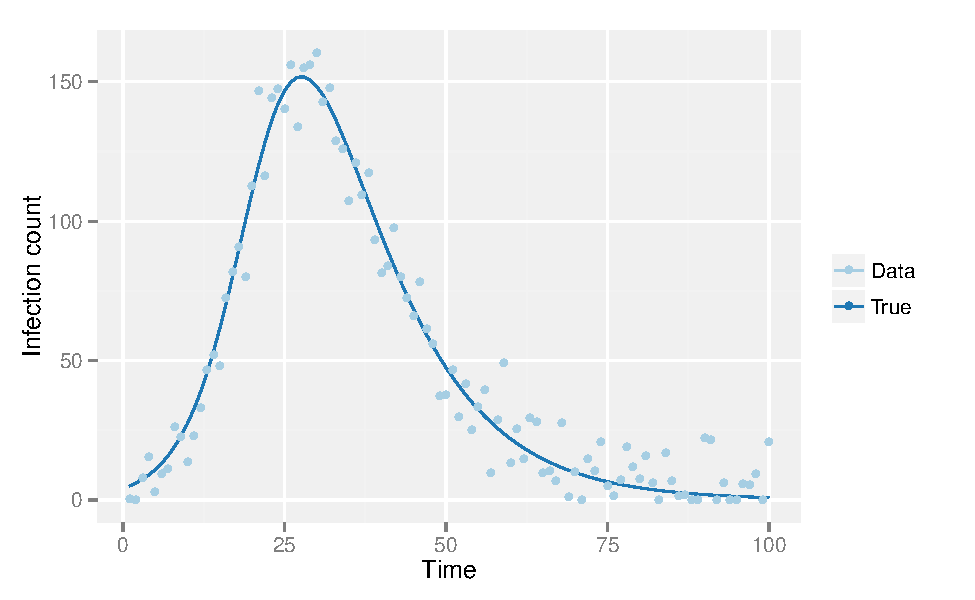
\includegraphics[width=\textwidth]{./images/dataplot.pdf}
        \caption{True SIR ODE solution infected counts, and with added observation noise}
        \label{dataplot}
    \end{figure}

    The IF2 algorithm was implemented in C++ for speed, and integrated into the R workflow using the \verb|Rcpp| package. The C++ code is compiled using

    \begin{R}
    sourceCpp(paste(getwd(),"if2.cpp",sep="/"))
    \end{R}

    Then run and packed into a data frame using

    \begin{R}
    paramdata <- data.frame(if2(infec_counts[1:Tlim], Tlim, N))
	  colnames(paramdata) <- c("R0", "r", "sigma", "Sinit", "Iinit", "Rinit")
    \end{R}

    The final kernel estimates for four of the key parameters are shown in Figure \ref{kernelplot}.

    \begin{figure}[H]
        \centering
        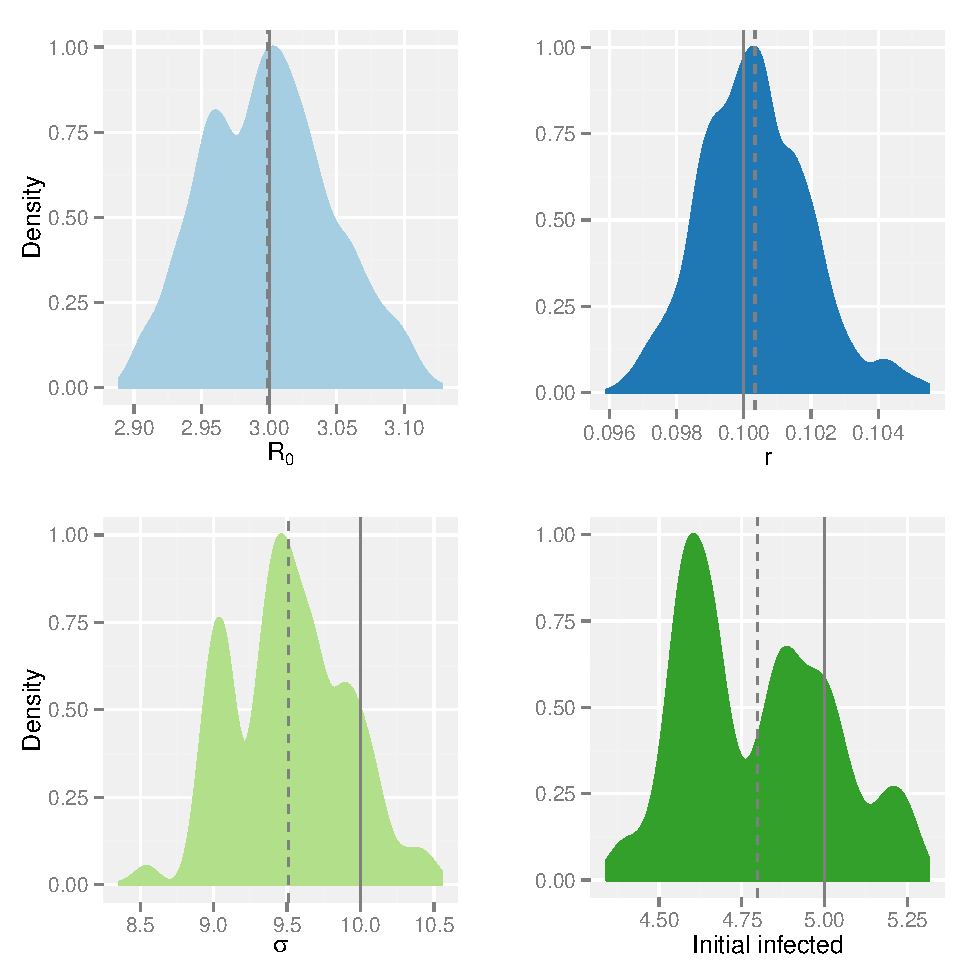
\includegraphics[width=\textwidth]{./images/if2kernels.pdf}
        \caption{Kernel estimates for four essential system parameters. True values are indicated by solid vertical lines, sample means by dashed lines.}
        \label{kernelplot}
    \end{figure}


	\chapter{Parameter Fitting}

		\graphicspath{{../SC1/}}
		%% Dexter Barrows, 2016
%% dbarrows.github.io

\section{Fitting Setup}

	Now that we have established which methods we wish to evaluate the efficacy of for epidemic forecasting, it is prudent to see how they perform when fitting parameters for a known epidemic model. We have already seen how they perform when fitting parameters for a model with a deterministic evolution process and observation noise, but a more realistic model will have both process and observation noise.

	To form such a model, we will take a deterministic SIR ODE model given by

	\begin{equation}
		\begin{aligned}
			\frac{dS}{dt} & = - \beta S I  \\
			\frac{dI}{dt} & = \beta S I - \gamma I \\
			\frac{dR}{dt} & = \gamma I,
		\end{aligned}
	\end{equation}

	and add process noise by allowing $\beta$ to embark on a geometric random walk given by

	\begin{equation}\label{betaautoreg}
		\beta_{t+1} = \exp \left( \log(\beta_{t}) + \eta (\log(\bar{\beta}) - \log(\beta_{t})) + \epsilon_{t} \right).
	\end{equation}

	We will take $\epsilon_{t}$ to be normally distributed with standard deviation $\rho^2$ such that $\epsilon_{t} \sim \mathcal{N}(0,\rho^2)$. The geometric attraction term constrains the random walk, the force of which is $\eta \in [0,1]$. If we take $\eta = 0$ then the walk will be unconstrained; if we let $\eta = 1$ then all values of $\beta_t$ will be independent from the previous value (and consequently all other values in the sequence).

	When $\eta \in (0,1)$, we have an autoregressive process of order 1 on the logarithmic scale of the form

	\begin{equation}
		X_{t+1} = c + \rho X_t + \epsilon_t ,
	\end{equation}

	where $\epsilon_t$ is normally distributed noise with mean 0 and standard deviation $\sigma_E$. This process has a theoretical expected mean of $\mu = c / (1 - \rho)$ and variance $\sigma = \sigma_E^2 / (1 - \rho^2)$. If we choose $\eta = 0.5$, the resulting log-normal distribution has a mean of $6.80 \times 10^{-4}$ and standard deviation of $4.46 \times 10^{-4}$.

	Simulating the process in Equation [\ref{betaautoreg}] with $\eta = 0.5$ gives us the plot in Figure [\ref{betaplot}].

	\begin{figure}
        \centering
        \captionsetup{width=.8\linewidth}
        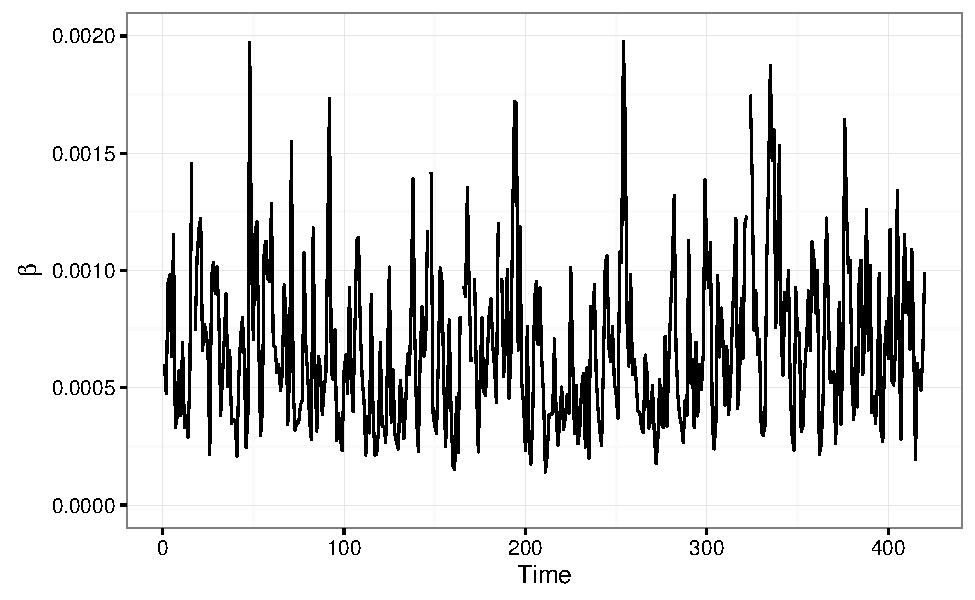
\includegraphics[width=0.8\textwidth]{./images/betaplot.pdf}
        \caption{Simulated geometric autoregressive process show in Equation [\ref{betaautoreg}]. \label{betaplot}}
    \end{figure}

    We can obtain the corresponding density plot of the values in Figure [\ref{betaplot}], shown in Figure [\ref{betadensity}].

    \begin{figure}
        \centering
        \captionsetup{width=.8\linewidth}
        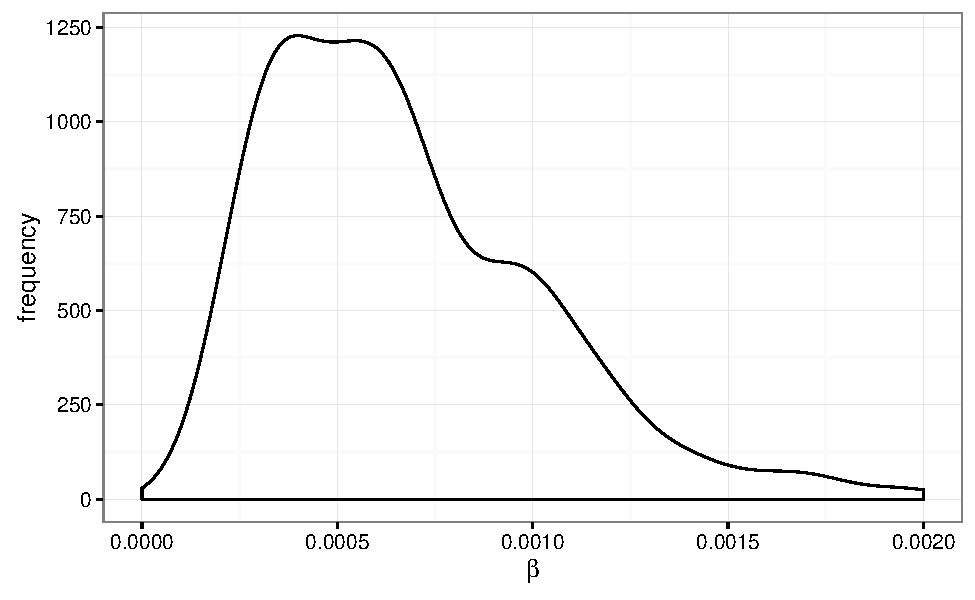
\includegraphics[width=0.8\textwidth]{./images/betadensity.pdf}
        \caption{Density plot of values shown if Figure[\ref{betaplot}]. \label{betadensity}}
    \end{figure}

    We see a density plot similar in shape to the desired density, and the geometric random walk displays dependence on previous values. Further the mean of this distribution was calculated to be $6.92 \times 10^{-4}$ and standard the deviation to be $3.99 \times 10^{-4}$, which are very close to the theoretical values.

    If we take the full stochastic SIR system and evolve it using an Euler stepping scheme with a step size of $h = 1/7$, for 1 step per day, we obtain the plot in Figure [\ref{sirmean}].

    \begin{figure}
        \centering
        \captionsetup{width=.8\linewidth}
        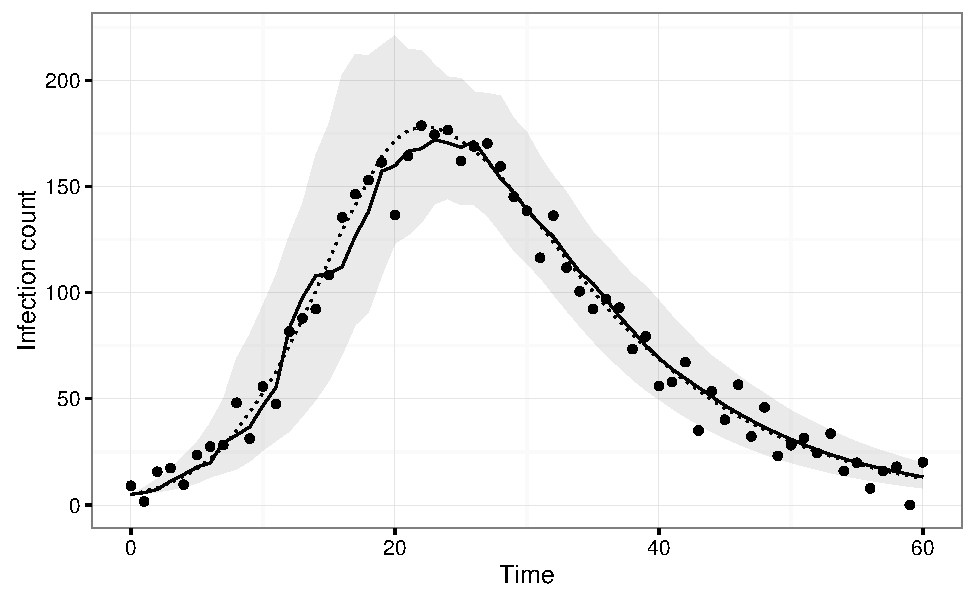
\includegraphics[width=0.8\textwidth]{./images/sirmean.pdf}
        \caption{Stochastic SIR model simulated using an explicit Euler stepping scheme. The solid line is a single random trajectory, the dots show the data points obtained by adding in observation error defined as $\epsilon_{obvs} = \mathcal{N}(0,10)$, and the grey ribbon is centre 95th quantile from 100 random trajectories. \label{sirmean}}
    \end{figure}


\section{Calibrating Samples}

	In order to compare HMCMC and IF2 we need to set up a fair and theoretically justified way to select the number of samples to draw for the HMCMC iterations and the number of particles to use for IF2. We assume that we are working with a problem that has an unknown real solution, so we use the Monte Carlo Standard Error (MCSE).

	Suppose we are using a Monte-Carlo based method to obtain an estimate $\hat{\mu}_{n}$ for a quantity $\mu$, where $n$ is the number of samples. Then the Law of Large Numbers says that $\hat{\mu}_{n} \rightarrow \mu$ as $n \rightarrow \infty$. Further, the Central Limit Theorem says that the error $\hat{\mu}_{n} - \mu$ should shrink with number of samples such that $\sqrt{n} (\hat{\mu}_{n} - \mu) \rightarrow \mathcal{N}(0,\sigma^2)$ as $n \rightarrow \infty$, where $\sigma^2$ is the variance of the samples drawn.

	We of course do not know $\mu$, but the above allows us to obtain an estimate $\hat{\sigma}_n$ for $\sigma$ given a number of samples $n$ as

	\begin{equation}
		\hat{\sigma}_n = \sqrt{\frac{1}{n} \sum_{i=1}^{n} (X_i - \hat{\mu}) },
	\end{equation}

	which is known as the Monte Carlo Standard Error.

	We can modify this formula to account for multiple variables by replacing the single variance measure sum by

	\begin{equation}
		\Theta^* V (\Theta^*)^T
	\end{equation}

	where $\Theta^*$ is a row vector containing the reciprocals of the means of the parameters of interest, and $V$ is the variance-covariance matrix with respect to the same parameters. This in effect scales the variances with respect to their magnitudes and accounts for covariation between parameters in one fell swoop. We also divide by the number of parameters, yielding

	\begin{equation}
		\hat{\sigma}_n = \sqrt{\frac{1}{n} \frac{1}{P} \Theta^* V (\Theta^*)^T }
	\end{equation}

	where $P$ is the number of particles.

	The goal here is to then pick the number of HMCMC samples and IF2 particles to yield similar MCSE values. To do this we picked a combination of parameters for RStan that yielded decent results when applied to the stochastic SIR model specified above, calculated the resulting mean MCSE across several model fits, and isolated the expected number of IF2 particles needed to obtain the same value. This was used as a starting value to ``titrate'' the IF2 iterations to the same point.

	The resulting values were 1000 HMCMC warm-up iterations with 1000 samples drawn post-warm-up, and 2500 IF2 particles sent through 50 passes, each method giving an approximate MCSE of 0.0065.


\section{IF2 Fitting}

	Now we will use an implementation of the IF2 algorithm to attempt to fit the stochastic SIR model to the previous data. The goal here is just parameter inference, but since IF2 works by applying a series on particle filters we essentially get the average system state estimates for a very small additional computational cost. Hence, we will will also look at that estimated behaviour in addition the the parameter estimates.

	The code used here is a mix of R and C++ implemented using RCpp. The fitting was undertaken using $2500$ particles with 50 IF2 passes and a cooling schedule given by a reduction in particle spread determined by $0.975^{p}$, where p is the pass number starting with 0.

	The MLE parameter estimates, taken to be the mean of the particle swarm values after the final pass, are shown in the table in Figure [\ref{fiterror}], along with the true values and the relative error.

	\begin{figure}[H]
		\centering
		{\small
		\begin{tabular}{cccccc}
			& & \multicolumn{2}{c}{IF2} & \multicolumn{2}{c}{HMCMC} \\
			\cmidrule[1.0pt](r){3-4} \cmidrule[1.0pt](r){5-6}
			Name & True	& Fit & Error & Fit & Error \\
			\cmidrule[1.0pt](r){1-1} \cmidrule[1.0pt](r){2-2} \cmidrule[1.0pt](r){3-3} \cmidrule[1.0pt](r){4-4} \cmidrule[1.0pt](r){5-5} \cmidrule[1.0pt](r){6-6}
			$R_0$ 				& 3.0 				 & 3.27 					& $9.08 \times 10^{-2}$ 	& $3.12$ 				& $1.05 \times 10^{-1}$		\\
			$r$ 				& $10^{-1}$  		 & $1.04 \times 10^{-1}$ 	& $3.61 \times 10^{-2}$ 	& $9.99 \times 10^{-2}$ & $-7.56 \times 10^{-4}$	\\
			Initial Infected 	& 5  				 & 7.90 					& $5.80 \times 10^{-1}$ 	& $6.64$ 				& $3.28 \times 10^{-1}$ 	\\
			$\sigma$ 			& 10   				 & 8.84 					& $-1.15 \times 10^{-1}$ 	& $8.5$ 				& $-1.50 \times 10^{-1}$	\\
			$\eta$ 				& $5 \times 10^{-1}$ & $5.87 \times 10^{-1}$ 	& $1.73 \times 10^{-1}$ 	& $4.57 \times 10^{-1}$ & $-8.27 \times 10^{-2}$ 	\\
			$\varepsilon_{err}$ & $5 \times 10^{-1}$ & $1.63 \times 10^{-1}$ 	& $-6.73 \times 10^{-1}$ 	& $1.60 \times10^{-1}$  & $-6.80 \times 10^{-1}$
		\end{tabular}}
	    \caption{Fitting errors. \label{fiterror}}
    \end{figure}


	From last IF2 particle filtering iteration, the mean state values from the particle swarm at each time step are shown with the true underlying state and data in the plot in Figure [\ref{if2state}].

	\begin{figure}
        \centering
        \captionsetup{width=.8\linewidth}
        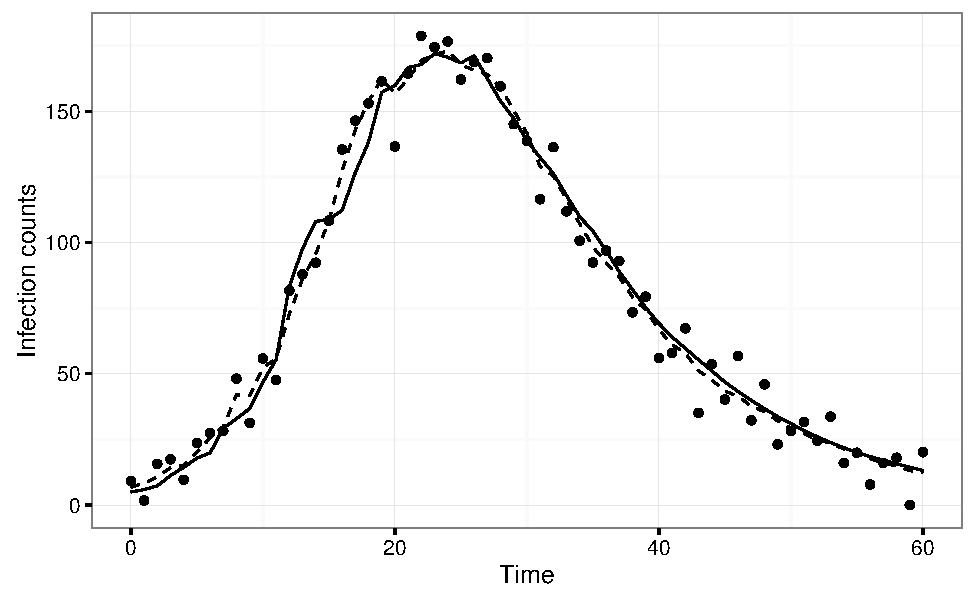
\includegraphics[width=0.8\textwidth]{./images/if2state.pdf}
        \caption{True system trajectory (solid line), observed data (dots), and IF2 estimated real state (dashed line). \label{if2state}}
    \end{figure}


\section{IF2 Convergence}

	Since IF2 is an iterative algorithm where each pass through he data is expected to push the parameter estimates towards the MLE, we can see the evolution of these estimates as a function of the pass number. Plots showing evolution of the mean estimates are shown if Figure [\ref{if2convergence}] for the six most critical parameters.

	\begin{figure}
        \centering
        \captionsetup{width=.8\linewidth}
        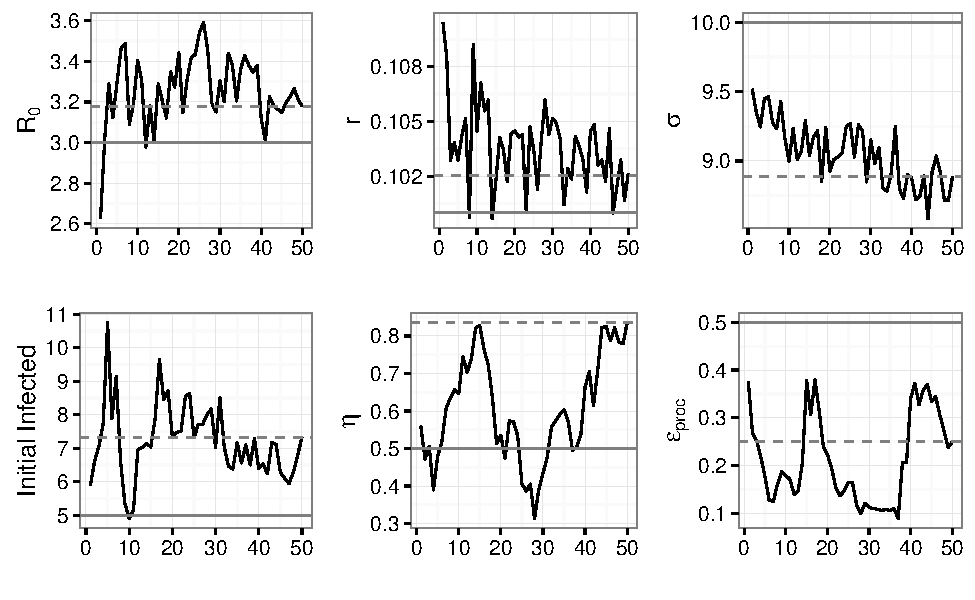
\includegraphics[width=0.8\textwidth]{./images/if2convergence.pdf}
        \caption{The horizontal axis shows the IF2 pass number. The solid black lines show the evolution of the ML estimates, the solid grey lines show the true value, and the dashed grey lines show the mean parameter estimates from the particle swarm after the final pass. \label{if2convergence}}
    \end{figure}

    Similarly, we can look at the evolution of the standard deviations of the parameter estimates from the particle swarm as a function of the pass number, shown in Figure [\ref{if2sdconvergence}].

    \begin{figure}
        \centering
        \captionsetup{width=.8\linewidth}
        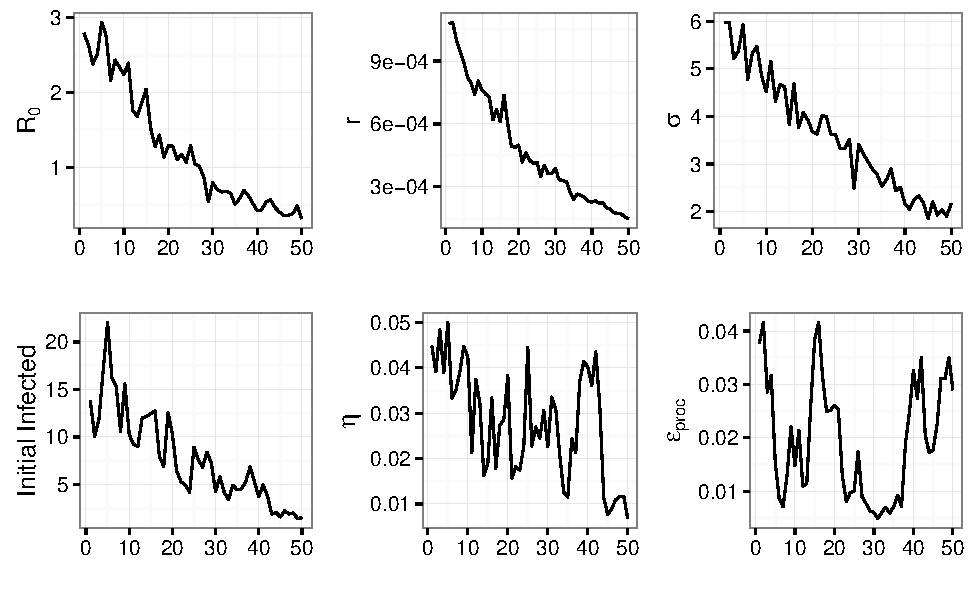
\includegraphics[width=0.8\textwidth]{./images/if2sdconvergence.pdf}
        \caption{The horizontal axis shows the IF2 pass number and the solid black lines show the evolution of the standard deviations of the particle swarm values. \label{if2sdconvergence}}
    \end{figure}

    As expected there is a downward trend in all plots, with a very strong trend in all but two of them.


\section{IF2 Densities}

	Of diagnostic importance are the densities of the parameter estimates given by the final parameter swarm. These are shown if Figure [\ref{if2kernels}].

	\begin{figure}
        \centering
        \captionsetup{width=.8\linewidth}
        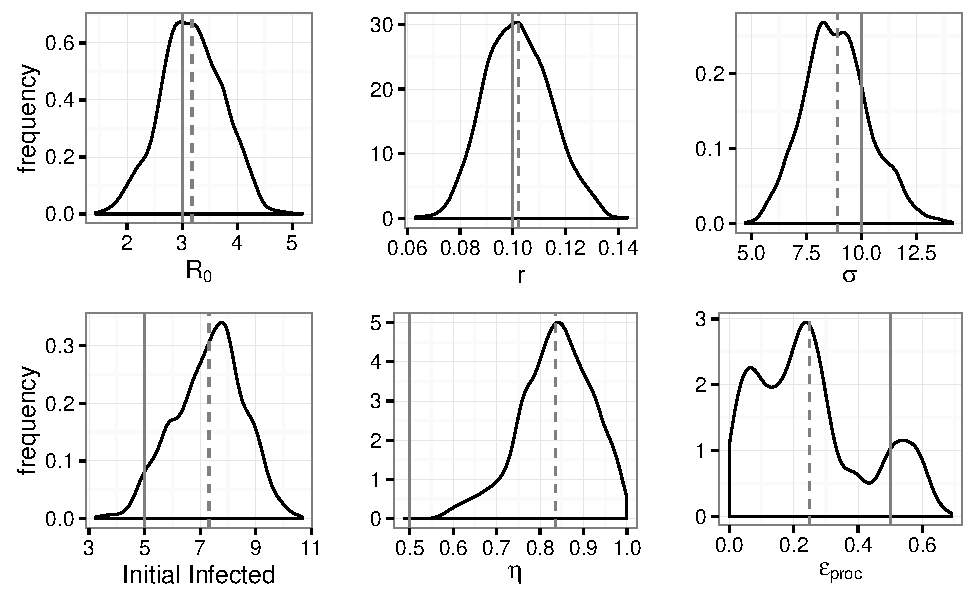
\includegraphics[width=0.8\textwidth]{./images/if2kernels.pdf}
        \caption{As before, the solid grey lines show the true parameter values and the dashed grey lines show the density means. \label{if2kernels}}
    \end{figure}

    It is worth noting that the IF2 parameters chosen were in part chosen so as to not artificially narrow these densities; a more aggressive cooling schedule and/or an increased number of passes would have resulted in much narrower densities, and indeed have the potential to collapse them to point estimates.


\section{HMCMC Fitting}

	We can use the Hamiltonian Monte Carlo algorithm implemented in the `Rstan` package to fit the stochastic SIR model as above. This was done with a single HMC chain of 2000 iterations with 1000 of those being warm-up iterations.

	The MLE parameter estimates, taken to be the means of the samples in the chain, were shown in the table in Figure [\ref{fiterror}] along with the true values and relative error.


\section{HMCMC Densities}

	The parameter estimation densities from the Stan HMCMC fitting are shown in Figure [\ref{hmckernels}].

	\begin{figure}
        \centering
        \captionsetup{width=.8\linewidth}
        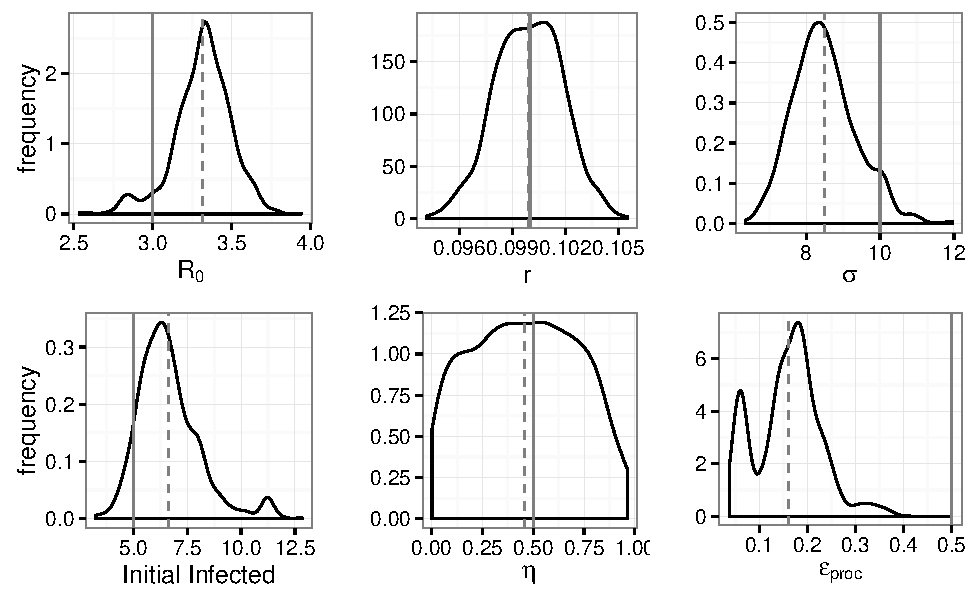
\includegraphics[width=0.8\textwidth]{./images/hmckernels.pdf}
        \caption{As before, the solid grey lines show the true parameter values and the dashed grey lines show the density means. \label{hmckernels}}
    \end{figure}

    the densities shown here represent a ``true'' MLE density estimate in that they represent HMC's attempt to directly sample from the parameter space according to the likelihood surface, unlike IF2 which is in theory only trying to get a ML point estimate. Hence, these densities are potentially more robust than those produced by the IF2 implementation.


\section{HMCMC and Bootstrapping}

	Unlike particle particle-filtering-based approaches, HMC does not produce state estimates as a by-product of parameter fitting, but we can use information about the stochastic nodes related to the noise in the $\beta$ geometric random walk to reconstruct state estimates. The results of 100 bootstrap trajectories is shown in Figure [\ref{hmcboot}].

	\begin{figure}
        \centering
        \captionsetup{width=.8\linewidth}
        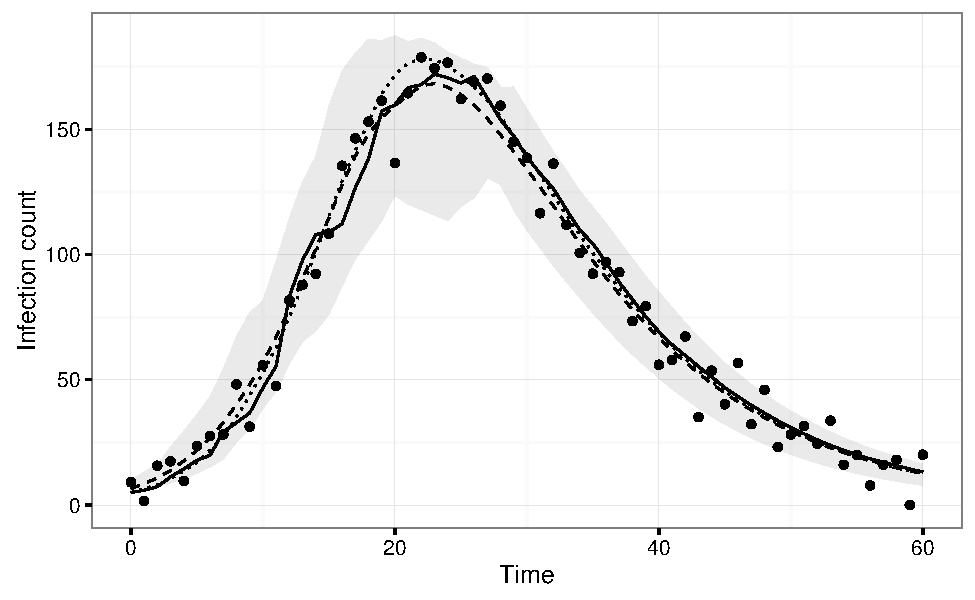
\includegraphics[width=0.8\textwidth]{./images/hmcboot.pdf}
        \caption{Result from 100 HMCMC bootstrap trajectories. The solid line shows the true states, the dots show the data, the dotted line shows the average system behaviour, the dashed line shows the bootstrap mean, and the grey ribbon shows the centre 95th quantile of the bootstrap trajectories. \label{hmcboot}}
    \end{figure}


\section{Multi-trajectory Parameter Estimation}

	Here we fit the stochastic SIR model to 200 random independent trajectories using each method and examine the density of the point estimates produced. 

    \begin{figure}
        \centering
        \captionsetup{width=.8\linewidth}
        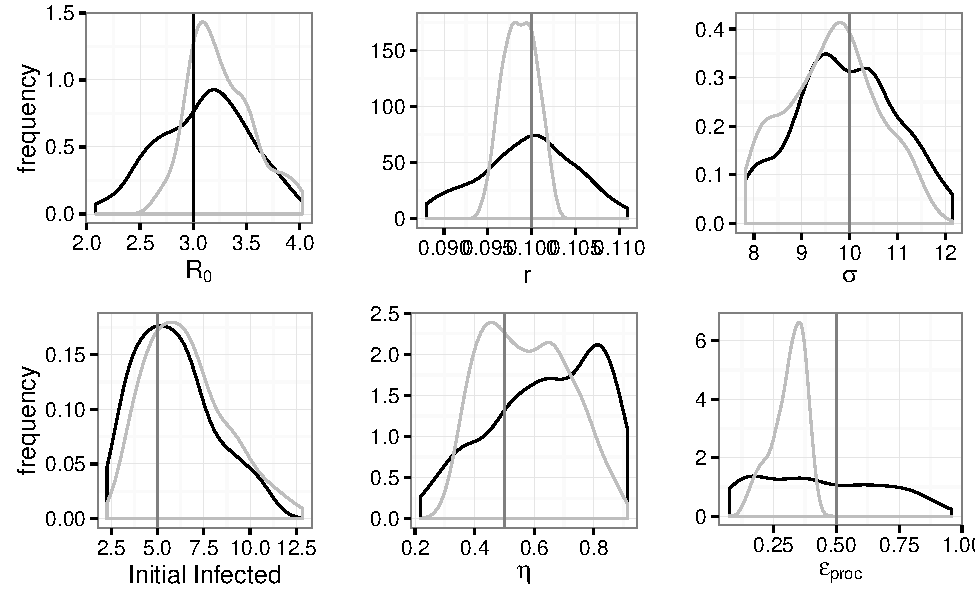
\includegraphics[width=0.8\textwidth]{./images/combined-multi.pdf}
        \caption{IF2 point estimate densities are shown in black and HMCMC point estimate densities are shown in grey. The vertical black lines show the true parameter values. \label{combinedmulti}}
    \end{figure}

    The densities by and large display similar coverage, with the IF2 densities for $r$ and $\varepsilon_{proc}$ showing slightly wider coverage than the HMCMC densities for the same parameters.

    The running times for each algorithm are summarized in Figure [\ref{timeplot}].

	\begin{figure}
        \centering
        \captionsetup{width=.8\linewidth}
        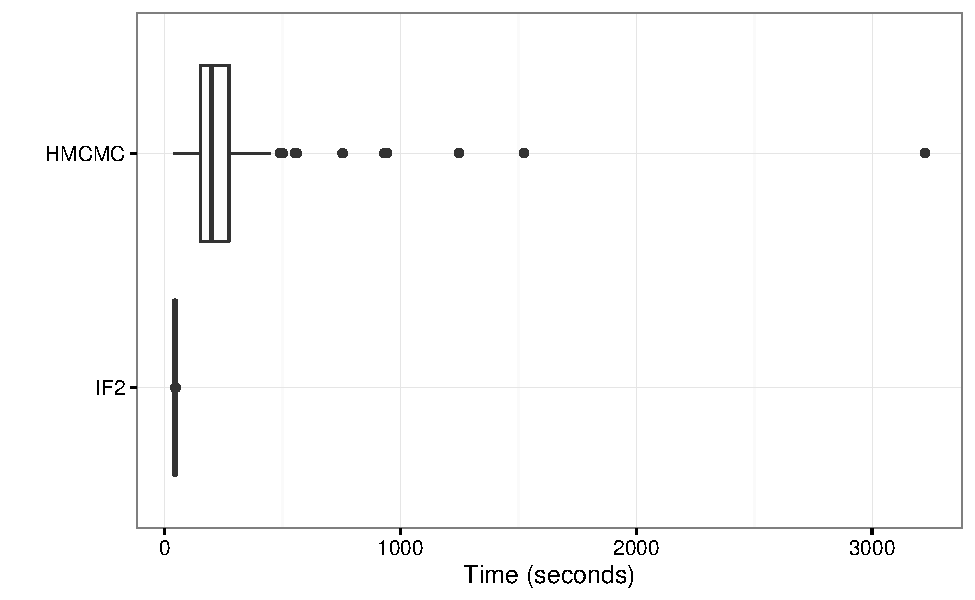
\includegraphics[width=0.8\textwidth]{./images/timeplot.pdf}
        \caption{Fitting times for IF2 and HMCMC, in seconds. The centre box in each plot shows the centre 50th quantile, with the bold centre line showing the median. \label{timeplot}}
    \end{figure}

    The average running times were approximately 45.5 seconds and 257.4 seconds for IF2 and HMCMC respectively, representing a 5.7x speedup for IF2 over HMCMC. While IF2 may be able to fit the model to data faster than HMCMC, we are obtaining less information; this will become important in the next section. Further, the results in Figure [\ref{timeplot}] show that while the running time for IF2 is relatively fixed, the times for HMCMC are anything but, showing a wide spread of potential times.


	\chapter{Forecasting Frameworks}

		\subfile{../SC2/sc2-text}

	\chapter{S-map and SIRS}

		\subfile{../SIRS-SMAP/sirs-smap-text}

	\chapter{Spatial Epidemics}

		\subfile{../SPATIAL/spatial-text}

	\chapter{Discussion and Future Directions}

		\subfile{../future-directions/future-directions}
	
	%% --------------------------------------------------------------------
	%% --------------------------------------------------------------------
	
	\nocite{*}
	\printbibliography

	%% --------------------------------------------------------------------
	%% --------------------------------------------------------------------

	\appendix

	\chapter{Hamiltonian MCMC}

		\subfile{../MCMC-HMCMC/mcmc-appendix}

	\chapter{Iterated Filtering}

		\subfile{../PF-IF2/pf-appendix}

	\chapter{Parameter Fitting}

		\subfile{../SC1/sc1-appendix}

	\chapter{Forecasting Frameworks}

		\subfile{../SC2/sc2-appendix}

	\chapter{S-map and SIRS}

		\subfile{../SIRS-SMAP/sirs-smap-appendix}

	\chapter{Spatial Epidemics}

		\subfile{../SPATIAL/spatial-appendix}

		\subfile{../SPATIAL/cuda-appendix}


	\end{linenumbers}
	

\end{document}

